\input{../header.tex}

\subject{VERSUCH NUMMER 64}
\title{Moderne Interferometrie}
\date{
  Durchführung: 29.04.2024
  \hspace{3em}
  Abgabe: DATUM
}

\begin{document}

\maketitle
\thispagestyle{empty}
\tableofcontents
\newpage
\setcounter{page}{1}
\section{Ziel}
\label{sec:Ziel}
\section{Theorie}
\label{sec:Theorie}

\subsection{Interferenz, Kohärenz und Polarisation}
\label{sec:polarisation}
Licht wird in diesem Versuch als stehende linearpolarisierte elektromagnetische Welle betrachtet, um Interferenzerscheinungen erklären zu können. Die elektrische Feldstärke ist 
ebenfalls eine solche Welle und kann über 
\begin{equation}
    \vec{E} = \vec{E}_0\cos{(\omega t+ \delta)}
    \label{eqn:EVektor}
\end{equation}
beschrieben werden. Die Ausbreitung von Licht wird dabei über die Maxwellschen Gleichungen beschrieben. Außerdem folgt das elektrische Feld 
$\vec{E}$ dem Prinzip der linearen Superposition. Somit ist die Welle in der x-z-Ebene polarisiert.
Die Intensität berechnet sich durch 
\begin{equation*}
    I = \langle E^2\rangle _{\text{T}} \; ,
\end{equation*}
wobei $\langle E^2\rangle _{\text{T}}$ nichts anderes als der zeitliche Mittelwert in einem Intervall T ist
\begin{equation}
    \langle f(t) \rangle _{\text{T}} = \frac{1}{T}\int_t^{t+T} f(t')\text{d}t \, .
    \label{eqn:zeitlichMittel}
\end{equation}
Da $E$ aus einer überlagerung von zwei Wellen besteht, wird $\vec{E}=(\vec{E}_1+\vec{E}_2)$ gesetzt, wodurch $\vec{E}^2= E_1^2+E_2^2+2\vec{E_1}\, \vec{E}_2\cdot\text{cos}(\alpha)$ folgt.
Der Winkel $\alpha$ ist hierbei der Winkelzwischen den beiden Wellen.
Bei einer Überlagerung von zwei Wellen ergibt sich für die Intensität 
\begin{equation*}
    I = I_1 +I_2 +I_{12}\; .
\end{equation*}
Der Ausdruck $I_{12}$ beschreibt hierbei den Interferenzterm.
Nimmt man an, dass $I_1=I_2$ gilt, so folgt, dass
wenn die Bedingung
\begin{equation*}
    \delta_2 -\delta_1 = \left(2n+1\right)\pi 
\end{equation*}
erfüllt ist, sich die Intensität zu null ergibt und
bei 
\begin{equation*}
    \delta_2 -\delta_1 = \left(2n\right)\pi 
\end{equation*}
sich ein Intesitätsmaximum der Stärke $I=4I_1cos^2{\left(\frac{\delta}{2}\right)}$ zeigt.

Bei zwei unabhängigen Lichtquellen, sind die Phasenkonstanten $\delta_1$ und $\delta_2$ statistische Funktionen der Zeit, wodurch es keine 
Interferenzerscheinung gibt. Dieses Licht ist dann inkohärent. Mithilfe eines LASERs (light amplification by stimulated emission of radiation)
ist es jedoch möglich kohärentes Licht zu erzeugen, welches ein festes $k$, $\omega$ und $\delta$ besitzt.
Bei einem Wegunterschied der einzelnen Strecken des Interferometers, der der Kohärenzlänge $l$ oder mehr entspricht, verschwindet jedoch die 
Interferenzerscheinung. Die Kohärenzlänge berechnet sich über
\begin{equation*}
    l = \text{N}\lambda \; .
\end{equation*}
Dabei ist N die Anzahl der bei beobachtbaren Intensitätsmaxima. Die Anzahl der beobachteten Maxima entsteht durch den Wegunterschied. Wenn der Welle ein Wegunterschied von $\Delta s=\lambda$ widerfährt, so ist ein Maximum erkennbar.Bei zweifachem Wegunterschied sind zwei Maxima detektierbar usw.
Diese Eigenschaft wird für die Bestimmung des Brechungsindex von Glas und Luft verwendet (siehe \autoref{sec:Durchführung}).

Eine weitere wichtige Eigenschaft für die Interferenz von Licht ist die Polarisation. Lichtpolarisation kann in vier Hauptkategorien unterteilt werden. Die erste ist die lineare Polarisation, bei der die Schwingungsrichtung des elektrischen Feldvektors in einer einzigen Ebene liegt.
 Darüber hinaus gibt es die zirkulare Polarisation. Hierbei rotiert die Schwingungsrichtung des elektrischen Feldvektors in einer kreisförmigen Bewegung. Die Schwingrichtung liegt folglich nicht mehr nur in einer Ebene. Zirkular Polarisiertes Licht kann weiter in zwei Unterkategorien unterteilt werden; links und
 rechtshändig polarisiert. Diese Polarisationsrichtung beschreibt die Richtung der Schwingung in Abhängigkeit zur Ausbreitungsrichtung 
Die dritte Möglichkeit ist die elliptische Polarisation, die eine Kombination aus linearer und zirkularer Polarisation ist. Bei dieser Art der Polarisation rotiert die Schwingungsrichtung des Feldvektors in einer elliptischen Bewegung.
Die letzte Möglichkeit ist unpolarisiertes Licht, welches sich durch keine geordnete Schwingungsrichtung auszeichnet.  
Drei der genannten Möglichkeiten sind in \autoref{fig:polarisation1} schematisch dargestellt.

\begin{figure}
    \centering
   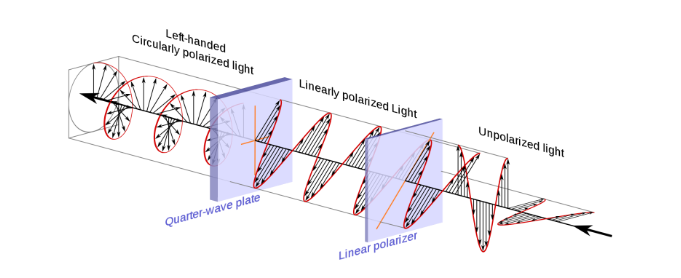
\includegraphics[width = 0.7 \linewidth]{Bilder/polarisation1.png}
    \caption{Drei der möglichen Polarisationsarten und Möglichkeiten diese ineinander umzuwandeln. \cite{Polarisation}.}
    \label{fig:polarisation1}
\end{figure}
Um ein Interferenzmuster zu erhalten, ist es nötig dass die Polarisationsrichtung der beiden Teilstrahlen nicht senkrecht aufeinander stehen. Für ein möglichst deutliches Interferenzmuster müssen beide Wellen die gleiche Polarisationsrichtung und -art haben.

\subsection{Kontrast} \label{sec:kontrast}
Als Kontrast (oder Sichtbarkeit) eines Interferometers wird die Beziehung
\begin{equation} \label{eqn:kontrast}
    V = \frac{I_\text{max} - I_\text{min}}{I_\text{max} + I_\text{min}}
\end{equation}
bezeichnet. Offensichtlich gilt also für den Kontrast: $V \in [0,1]$.
Hierbei beschreibt $V$ die Qualität und Deutlichkeit des Interferenzbildes. Hat $V$ den Wert 1, so ist das Minimum nicht sichtbar. Je stärker das Minimum sichtbar ist, desto kleiner wird $V$ bis es den Wert 0 erreicht und keine Interferenz mehr zu erkennen ist.
Aus zwei überlagerten Wellen $E=(E_1+E_2)$ folgt nach Einsetzen von \autoref{eqn:EVektor} in \autoref{eqn:zeitlichMittel} für die Intensität
\begin{equation*}
    I = \langle E^2\rangle _{\text{T}}= \frac{1}{T}\int_t^{t+T}  (\vec{E}_{0,1}\cos{(\omega t)})^2+(\vec{E}_{0,2}\cos{(\omega t+ \delta)})^2+2\vec{E}_{0,1}\cos{(\omega t)}\, \vec{E}_{0,2}\cos{(\omega t+ \delta)}\cdot\text{cos}(\alpha)\text{d}t\, .
\end{equation*}
Hierbei wurde die Phasenverschiebung $\delta$ als Verschiebung der zweiten zur ersten Welle definiert. Unter der Vereinfachung, dass sich die Welle nur entlang einer Achse ausbreitet, der Winkel zwischen den beiden Strahlen $\alpha=0$ ist und beide Wellen die gleiche Intensität haben folgt für die Intensität

\begin{equation*}
    I=\frac{1}{T}\int_t^{t+T} (E_{0}\cos{(\omega t)})^2+(E_{0,2}\cos{(\omega t+ \delta)})^2+2E_{0}\cos{(\omega t)}\, E_{0}\cos{(\omega t+ \delta)}\text{d}t\, .
\end{equation*}
Nach ausführen des Integrals und kann nach kurzer Umformung
folgende Beziehung für die Intensitätsmaxima/- und minima gefunden werden
\begin{equation*}
    I_\text{max/min} \propto I_\text{Laser} \left[ 1 \pm 2 \cos(\Phi) \sin (\Phi) \right] \, ,
\end{equation*}
aus der sich wiederrum mit \autoref{eqn:kontrast} die Gleichung
\begin{align}\label{eqn:kontrast2}
    V = V(\Phi) &\propto \left|\frac{\left[ 1 + 2 \cos(\Phi) \sin (\Phi) \right] - \left[ 1 - 2 \cos(\Phi) \sin (\Phi) \right]}{\left[ 1 + 2 \cos(\Phi) \sin (\Phi) \right] + \left[ 1 - 2 \cos(\Phi) \sin (\Phi) \right]}\right| \\
    &= \left|2 \cos(\Phi) \sin(\Phi) \right| = \left| \sin (2 \Phi) \right|
\end{align}
ergibt. %Hieraus ist auch sofort ersichtlich, dass der Kontrast bei ungefähr $45°$ am höchsten sein dürfte, wenn alle anderen Einflüsse optimiert sind.
Die Größe $\Phi$ ist hierbei der Polarisationswinkel. 
\subsection{Brechungsindex} \label{sec:n}

Der Brechungsindex ist eine intrinsische Eigenschaft eines Materials und kann mittels Interferometer bestimmt werden. Ein Medium mit einem Brechungsindex $n_\text{Medium} > 1$ reduziert die Geschwindigkeit des einfallenden Lichts, was durch die Gleichung
\begin{equation*}
    v_\text{Medium} = \frac{c}{n}
\end{equation*}
beschrieben wird. Ein Lichtstrahl, der durch ein Medium geleitet wird, erfährt eine Phasenverschiebung. Diese Phasenverschiebung kann in Interferometern genutzt werden, um den Brechungsindex eines Mediums zu bestimmen.

Für die Phasenverschiebung in Luft gilt
\begin{equation} \label{eq:nluft}
    \Delta \delta = \frac{2 \pi}{\lambda_\text{vac}} \Delta n \cdot L \, ,
\end{equation}
wobei $L$ die Länge der evakuierten Zelle ist. Durch Einsetzen der Beziehung der gezählten Intensitätsmaxima 
\begin{equation} \label{eq:maxima}
    M = \frac{\Delta \delta}{2 \pi}
\end{equation}
in \autoref{eq:nluft} lässt sich der Brechungsindex bestimmen:
\begin{align} \label{eq:nluft2}
    \Delta n &= n_\text{Luft} - n_\text{Vak} = \frac{M \cdot \lambda_\text{vac}}{L} \nonumber \\
    n_\text{Luft} &= \frac{M \cdot \lambda_\text{vac}}{L} + 1
\end{align}

Mithilfe des Lorentz-Lorenz-Gesetzes lässt sich der Brechungsindex unter Normalbedingungen berechnen. Das Lorentz-Lorenz-Gesetz lautet
\begin{equation*}
    \frac{n^2 - 1}{n^2 + 2} = \frac{A p}{R T} \, ,
\end{equation*}
wobei $A$ die Refraktivität beschreibt und $R$ die allgemeine Gaskonstante. Nach einer Taylorentwicklung ergibt sich
\begin{equation*}
    n(p) \approx \frac{2 (n-1)}{3} \, ,
\end{equation*} 
woraus sich dann
\begin{equation} \label{eq:lorentz}
    n (T,p) \approx \frac{3 A p}{ 2 R T} + 1
\end{equation}
ergibt. Die Größe $T$ ist hierbei die Temperatur.

In diesem Experiment wird auch der Brechungsindex von Glas bestimmt. Für den Brechungsindex in Glas gilt
\begin{equation}\label{eq:phiglas}
    \Delta \delta = \frac{2\pi}{\lambda}T\left(\frac{n-1}{2n}\Delta \theta^2+O( \Delta \theta^4)\right) \, .
\end{equation}
Hierbei ist $T$ die Dicke des Glasplättchens.
Diese Gleichung wird modifiziert, da zwei Glasplättchen verbaut sind und um $\theta_0 = \pm 0.175\,\text{rad}$ verkippt sind. Damit ergibt sich die Gleichung in führender Ordnung
\begin{equation}
    \Delta \delta = \frac{\pi \cdot (n - 1) T}{\lambda \cdot n} \left(\left( \theta + 0.175 \right)^2 - \left( \theta - 0.175 \right)^2\right) \, ,
\end{equation}
was mit \autoref{eq:maxima} auf die Gleichung
\begin{equation*}
    M = \frac{n - 1}{\lambda \cdot n} \cdot 2 \theta \cdot |\theta_0|
\end{equation*}
und somit auf
\begin{equation} \label{eq:n_Glas}
    n = \frac{1}{1- \frac{\lambda M}{ 2 \theta \cdot |\theta_0| T}}
\end{equation}
führt.
\section{Aufbau}
\label{sec:Aufbau}
In diesem Versuch wird ein Sagnac-Interferometer verwendet. Dieses ist in \autoref{fig:Sagnac}
schematisch dargestellt. 
\begin{figure}
    \centering
    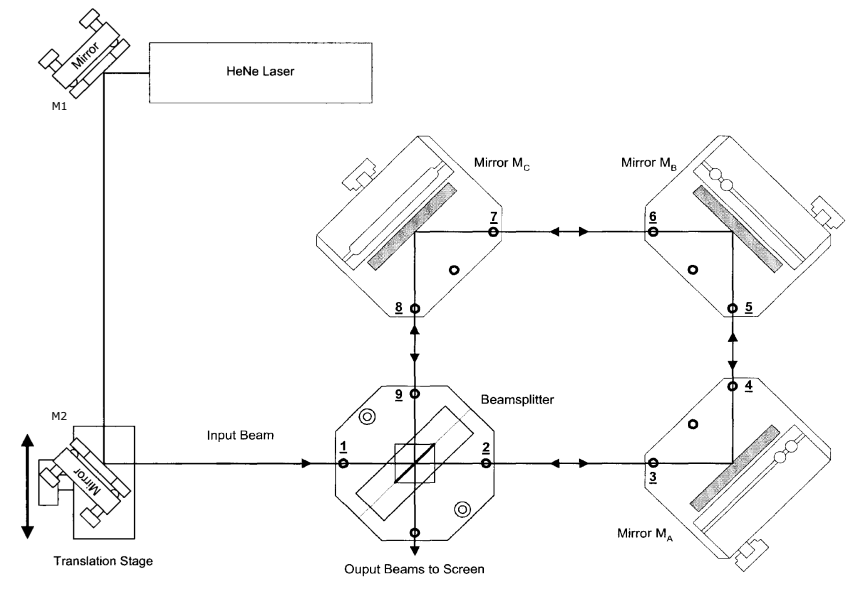
\includegraphics[width=0.8\textwidth]{Sagnac.png}
    \caption{Schematischer Aufbau eines Sagnac-Interferometers \cite{ap64}.}
    \label{fig:Sagnac}
\end{figure}
Das Interferometer besteht aus einem HeNe-Laser, der linear polarisiertes Licht der Wellenlänge $632.99\,\unit{\nano\meter}$
emittiert, und aus mehreren Spiegeln. Das Licht des Lasers ist in dessen Polarisation außerdem um 45° gegenüber der Vertikalen gekippt.
Die ersten beiden Spiegel M1 und M2 dienen dazu, den Laser in das Interferometer zu lenken. Die weiteren drei Spiegel $\symup{M_A}$, 
$\symup{M_B}$ und $\symup{M_C}$ sind Teil des Interferometers. Des Weiteren enthält es ein PBSC, der den Laserstrahl teilt.
Zur Justage liegen dem Versuch 2 Justageplatten sowie Metallplättchen bei. Außerdem stehen ein Schirm, ein 45°-Polarisationsfilter und ein um 45°-gedrehter
PBSC zur Verfügung. 
Für die Messung enthält der Versuch zwei verkippte dünne Glasplatten mit der Dicke $T=1\,\mathrm{mm}$, eine Gaszelle, Photodioden sowie
ein Oszilloskop.
\section{Durchführung}
\label{sec:Durchführung}
Der Versuch beginnt damit, die einzelnen Bauteile genau zu justieren. Hier wird auf diesen Prozess nicht genauer eingegangen, dieser ist in der Versuchsanleitung
\cite{ap64} beschrieben. \\
\\
Zuerst wird der Kontrast des Interferometers in Abhängigkeit von der Polarisationsrichtung $\phi$ des Laserstrahls gemessen. Dazu werden das Interferenzmaximum und -minimum
mittels einer Photodiode gemessen. Das Interferenzmaximum und -minimum kann durch den Doppelglashalter eingestellt werden.
Die Diodenspannung wird in Abhängigkeit von der Orientierung des Polarisationsfilters vor dem ersten PBSC gemessen. Dazu wird je im Abstand von 5° eine Messung aufgenommen.
\\
\\
Nun werden die Brechungsindizes von Glas und Luft vermessen. Dazu wird der Polarisator so eingestellt, dass der Kontrast maximal ist. 
Um den Brechungsindex von Glas zu bestimmen, wird die Anzahl der Interferenzmaxima in Abhängigkeit vom Drehwinkel 
$\theta$ der Glasplatten aus dem Doppelglashalter gemessen. Die Messung wird insgesamt zehnmal durchgeführt, um ein genaueres Ergebnis zu erhalten. \\
\\
Um den Brechungsindex von Luft zu messen, wird eine Gaszelle in einen Strahl eingebaut, 
In die zuvor evakuierte Gaszelle wird nun Luft eingeleitet. Dann wird die Anzahl der Interferenzmaxima in 
Abhängigkeit vom Druck gemessen. Dazu wird er Druck in $50\,\mathrm{mbar}$-Schritten erhöht. Es wird außerdem die Raumtemperatur notiert. Die Messung des Brechungsindex 
von Luft wird zur besseren Genauigkeit dreimal wiederholt.
\section{Auswertung}
\label{sec:Auswertung}

\subsection{Fehlerrechnung}
\label{sec:Fehlerrechnung}
Für die Fehlerrechnung werden folgende Formeln aus der Vorlesung verwendet.
für den Mittelwert gilt
\begin{equation}
    \overline{x}=\frac{1}{N}\sum_{i=1}^N x_i ß\; \;\text{mit der Anzahl N und den Messwerten x} 
    \label{eqn:Mittelwert}
\end{equation}
Der Fehler für den Mittelwert lässt sich gemäß
\begin{equation}
    \increment \overline{x}=\frac{1}{\sqrt{N}}\sqrt{\frac{1}{N-1}\sum_{i=1}^N(x_i-\overline{x})^2}
    \label{eqn:FehlerMittelwert}
\end{equation}
berechnen.
Wenn im weiteren Verlauf der Berechnung mit der fehlerhaften Größe gerechnet wird, kann der Fehler der folgenden Größe
mittels Gaußscher Fehlerfortpflanzung berechnet werden. Die Formel hierfür ist
\begin{equation}
    \increment f= \sqrt{\sum_{i=1}^N\left(\frac{\partial f}{\partial x_i}\right)^2\cdot(\increment x_i)^2}.
    \label{eqn:GaussMittelwert}
\end{equation}

\subsection{Kontrast}

\begin{sidewaystable}
\begin{tabular}{c c c c c c c c c c}
    \toprule
        Winkel/°&\multicolumn{3}{c}{Minima/V}&Mittelwert der Minima&\multicolumn{3}{c}{Maxima/V}&Mittelwert der Maxima&Kontrast \\
    \midrule
      0& 1.55 & 1.48 & 1.48 & 1.50 & 1.83 & 1.78 & 1.78 & 1.80 & 0.089 \\
      5& 1.26 & 1.26 & 1.27 & 1.26 & 1.53 & 1.58 & 1.59 & 1.57 & 0.107 \\
     10& 1.04 & 1.01 & 0.98 & 1.01 & 1.56 & 1.55 & 1.55 & 1.55 & 0.212 \\
     15& 0.67 & 0.68 & 0.68 & 0.68 & 1.56 & 1.56 & 1.53 & 1.55 & 0.392 \\
     20& 0.47 & 0.48 & 0.49 & 0.48 & 1.48 & 1.49 & 1.45 & 1.47 & 0.509 \\
     25& 0.30 & 0.31 & 0.32 & 0.31 & 1.46 & 1.47 & 1.41 & 1.45 & 0.647 \\
     30& 0.21 & 0.19 & 0.18 & 0.19 & 1.30 & 1.34 & 1.39 & 1.34 & 0.748 \\
     35& 0.11 & 0.10 & 0.10 & 0.10 & 1.40 & 1.41 & 1.42 & 1.41 & 0.863 \\
     40& 0.07 & 0.07 & 0.09 & 0.08 & 1.47 & 1.47 & 1.44 & 1.46 & 0.900 \\
     45& 0.05 & 0.05 & 0.07 & 0.06 & 1.53 & 1.52 & 1.52 & 1.52 & 0.928 \\
     50& 0.05 & 0.06 & 0.04 & 0.05 & 1.71 & 1.69 & 1.71 & 1.70 & 0.943 \\
     55& 0.07 & 0.07 & 0.08 & 0.07 & 1.81 & 1.81 & 1.81 & 1.81 & 0.922 \\
     60& 0.15 & 0.13 & 0.15 & 0.14 & 1.94 & 1.91 & 1.92 & 1.92 & 0.861 \\
     65& 0.21 & 0.21 & 0.21 & 0.21 & 2.07 & 2.03 & 2.05 & 2.05 & 0.814 \\
     70& 0.40 & 0.40 & 0.43 & 0.41 & 2.33 & 2.33 & 2.39 & 2.35 & 0.703 \\
     75& 0.69 & 0.62 & 0.62 & 0.64 & 2.20 & 2.26 & 2.26 & 2.24 & 0.554 \\
     80& 1.01 & 0.97 & 0.96 & 0.98 & 2.10 & 2.20 & 2.21 & 2.17 & 0.378 \\
     85& 1.34 & 1.26 & 1.26 & 1.29 & 1.97 & 2.15 & 2.15 & 2.09 & 0.238 \\
     90& 1.78 & 1.71 & 1.75 & 1.75 & 2.06 & 2.07 & 2.15 & 2.09 & 0.090 \\
     95& 1.91 & 1.91 & 1.92 & 1.91 & 2.44 & 2.53 & 2.53 & 2.50 & 0.133 \\
    100& 1.62 & 1.46 & 1.45 & 1.51 & 3.14 & 3.12 & 3.14 & 3.13 & 0.350 \\
    105& 1.19 & 1.15 & 1.16 & 1.17 & 3.66 & 3.68 & 3.65 & 3.66 & 0.517 \\
    110& 1.01 & 0.89 & 0.88 & 0.93 & 4.39 & 4.43 & 4.41 & 4.41 & 0.653 \\
    115& 0.60 & 0.60 & 0.60 & 0.60 & 4.86 & 4.85 & 4.85 & 4.85 & 0.780 \\
    120& 0.41 & 0.40 & 0.40 & 0.40 & 5.45 & 5.44 & 5.45 & 5.45 & 0.862 \\
    125& 0.23 & 0.21 & 0.22 & 0.22 & 5.85 & 5.82 & 5.87 & 5.85 & 0.927 \\
    130& 0.15 & 0.15 & 0.15 & 0.15 & 5.98 & 6.01 & 6.03 & 6.01 & 0.951 \\
    135& 0.15 & 0.14 & 0.15 & 0.15 & 5.90 & 5.90 & 5.99 & 5.93 & 0.952 \\
    140& 0.22 & 0.23 & 0.22 & 0.22 & 5.94 & 5.94 & 5.94 & 5.94 & 0.928 \\
    145& 0.63 & 0.35 & 0.32 & 0.43 & 5.40 & 5.31 & 5.31 & 5.34 & 0.850 \\
    150& 0.55 & 0.51 & 0.52 & 0.52 & 5.11 & 5.09 & 5.10 & 5.10 & 0.813 \\
    155& 0.79 & 0.77 & 0.79 & 0.78 & 4.30 & 4.48 & 4.46 & 4.41 & 0.699 \\
    160& 0.97 & 0.96 & 0.96 & 0.96 & 3.98 & 3.95 & 3.96 & 3.96 & 0.609 \\
    165& 1.13 & 1.14 & 1.13 & 1.13 & 3.15 & 3.19 & 3.14 & 3.16 & 0.472 \\
    170& 1.33 & 1.33 & 1.34 & 1.33 & 2.78 & 2.78 & 2.78 & 2.78 & 0.352 \\
    175& 1.48 & 1.47 & 1.47 & 1.47 & 2.27 & 2.26 & 2.25 & 2.26 & 0.211 \\
    180& 1.51 & 1.50 & 1.50 & 1.50 & 1.69 & 1.69 & 1.68 & 1.69 & 0.057 \\
    \bottomrule
    \end{tabular}
    \label{tab:kontrast}
\end{sidewaystable}

\begin{figure}
    \centering
    \includegraphics[width=0.8\textwidth]{build/kontrast.pdf}
    \caption{Kontrast in Abhängigkeit vom Winkel des Polarisationsfilters.}
    \label{fig:kontrast}
\end{figure}

\subsection{Brechungsindex von Glas}
\label{sec:AuswGlas}
Die Anzahl der Peaks und die aus \autoref{eqn:Brechi} resultierenden Brechindizes sind in \autoref{tab:Glasn} dargestellt.
\begin{table}
    \centering
    \caption{Anzahl der Peaks und der daraus resultierende Brechungsindex.}
    \begin{tabular}{c c c}
        \toprule
        Messung & Anzahl der Minima & Brechungsindex $n$ \\
        \midrule
             1 & 34 & 1.546\\
             2 & 34 & 1.546\\
             3 & 35 & 1.571\\
             4 & 35 & 1.571\\
             5 & 34 & 1.546\\
             6 & 34 & 1.546\\
             7 & 36 & 1.597\\
             8 & 34 & 1.546\\
             9 & 35 & 1.571\\
            10 & 33 & 1.522\\
            \bottomrule
    \end{tabular}
    \label{tab:Glasn}
\end{table}
Der daraus resultierende Mittelwert für den Brechungsindex $n$ von Glas beträgt $n=1.556$.


\subsection{Brechungsindex von Luft}
\label{sec:AusLuft}
In diesem Teil der Auswertung wird der Brechungsindex von Luft ermittelt. Die Daten der Messreihen sind in \autoref{tab:Brechung} niedergeschrieben und in \autoref{fig:allefüreinen} graphisch aufgetragen.
\begin{table}
    \centering
    \caption{Messwerte zur Messung des Brechungsindex von Luft.}
\begin{tabular}{c c c c c c c c }
    \toprule
    Druck $p \mathrm{/} \unit{\milli \bar}$ & Messung 1& Messung 2& Messung 3& Messung 4& Messung 5& Mittelwert \\
    \midrule
                           50& 3& 2& 2& 2& 2& 2.2 \\
                          100& 5& 4& 4& 4& 4& 4.2 \\
                          150& 7& 6& 6& 6& 6& 6.2 \\
                          200& 9& 8& 8& 8& 8& 8.2 \\
                    250& 11& 10& 10& 10& 10& 10.2 \\
                    300& 13& 12& 12& 12& 12& 12.2 \\
                    350& 15& 14& 14& 15& 14& 14.4 \\
                    400& 17& 16& 17& 17& 17& 16.8 \\
                      450& 19& 19& 19& 19& 19& 19 \\
                    500& 22& 21& 21& 21& 21& 21.2 \\
                    550& 24& 23& 23& 23& 23& 23.2 \\
                    600& 26& 25& 25& 25& 25& 25.2&  \\
                    650& 28& 27& 27& 27& 27& 27.2 \\
                    700& 30& 29& 29& 29& 29& 29.2 \\
                    750& 32& 31& 31& 31& 31& 31.2 \\
                    800& 35& 33& 33& 34& 34& 33.8 \\
                    850& 37& 36& 37& 36& 36& 36.4 \\
                    900& 39& 38& 39& 38& 38& 38.4 \\
                    950& 41& 40& 41& 40& 40& 40.4 \\
                   1000& 43& 42& 43& 42& 42& 42.4 \\
    \bottomrule
    \end{tabular}
    \label{tab:Brechung}
\end{table}

\begin{figure}
    \centering
    \includegraphics[height = 6cm]{build/luft.pdf}
    \caption{Messwerte der fünf Messungen zur Bestimmung von $n$.}
    \label{fig:allefüreinen}
\end{figure}
Um aus den Messwerten ein Brechungsindex ermitteln zu können, wird der Durchschnitt der fünf Messungen für den jeweiligen Druck ermittelt und aufgetragen. Die anschließend durchgeführte lineare Regression nach \autoref{eq:nluft2} mit $T=293.75\,\unit{\kelvin}$
liefert die in blau eingezeichnete Ausgleichsgerade mit einem Wert von $M=0.0780\pm 0.0005$.
Dieser Plot ist in \autoref{fig:einerfüralle} dargestellt.
\begin{figure}
    \centering
    \includegraphics[height = 6cm]{build/luftavg.pdf}
    \caption{Durchschnitt der fünf Messungen und lineare Regression.}
    \label{fig:einerfüralle}
\end{figure}

\section{Diskussion}
\label{sec:Diskussion}

Der Verlauf der Messwerte des Kontrasts in \autoref{fig:kontrast} liegen sehr nah an der Theoriekurve. Außerdem konnten sehr große Maxima 
des Kontrasts bei $K=0.943$ bei $\phi=50°$ und bei $K=0.952$ bei $\phi = 135°$ gemessen werden. Theoretisch wird das Maximum bei $45°$ 
erwartet. Die Abweichung dazu liegt in unserer Messung bei $11.11\%$. Diese lässt sich daraus erklären, dass zum einen nur im Abstand von 
$5°$ gemessen wurde und es so möglich ist, dass es ein Maximum gibt, dass dichter an dem theoretischen Wert liegt. Außerdem lässt sich die 
Abweichung dadurch erklären, dass das Interferometer nicht perfekt justiert war. Bereits kleine Erschütterungen ließen die Spiegel verrücken.

Der Brechungsindex von Glas liegt bei circa 1.5. Dieser variiert je nach Glas.
 Wenn dies mit unserer Messung $n=1.556$ verglichen wird, kann festgestellt werden, dass es keine Abweichung gibt. Dies zeigt, dass die Messung 
sehr genau durchgeführt wurde. Die Abdeckung über dem Interferometer konnte Fluktuationen abschirmen.

Der Brechungsindex von Luft liegt bei 20°C bei $n=1.00029$. Bei 15°C liegt dieser bei 1.00028, sodass sich erkennen lässt, dass der Brechungsindex 
mit der Temperatur minimal ansteigt. Dennoch ergibt sich eine Abweichung zu unserem gemessenen Wert von $4.1\%$. Diese lässt sich damit erklären, 
dass die Zusammensetzung von Luft nicht an jedem Ort gleich ist und für den Theoriewert ein Durchschnittswert angenommen wird. Außerdem 
ließ sich die Anzahl der Maxima nicht so gut in der Abhängigkeit vom Druck ablesen. Auch Fluktuationen innerhalb des Interferometers konnten nicht 
gänzlich ausgeschlossen werden.

\newpage
\printbibliography
\nocite{ap64}
\nocite{matplotlib}
\nocite{numpy}
\nocite{scipy}
\nocite{uncertainties}
\nocite{reback2020pandas}

\newpage
%\includepdf[scale=0.7,pages=1,pagecommand=\section*{Anhang}\thispagestyle{empty}]{messdaten.pdf}
%\addcontentsline{toc}{section}{\protect\numberline{}Anhang}
%\includepdf[scale = 0.7, pages=-]{messdaten.pdf}

\end{document}
